\begin{figure*}[htb]
\vskip 0.2in
\begin{center}
\centerline{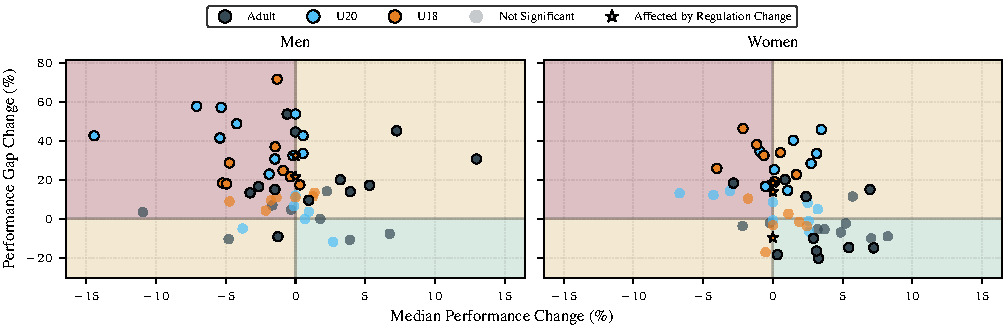
\includegraphics[width=\textwidth]{figures/gap_performance_change.pdf}}
\caption{Change in median performance vs. performance gap (2001–2005 to 2021–2025, in \%) for men and women across age groups. Marker transparency denotes statistical significance for performance gap (p < 0.05). Median changes for disciplines with regulatory updates are fixed at zero due to restricted comparability.
}
\label{gap_perf}
\end{center}
\vskip -0.2in
\end{figure*}

Figure \ref{gap_perf} shows the change in performance spread and typical performance development from 2021-2025 compared to 2001-2005 in many groups. 
The analysis of the performance data encompasses 106 groups, where X groups were excluded for median calculations (see Section \ref{sec:methods}). Overall, a decrease in performance density is evident. The best performers are improving, while the weaker performers are declining.
While median performance trends were nearly balanced with 38 groups significantly improving and 37 declining, the performance spread shows a strong asymmetry: A significant expansion was observed in 49.1\% (52 groups), while a reduction was only seen in 4.7\% (6 groups). This widening of the performance gap was most pronounced among men, especially in the U20 (70.6\%) age group. In contrast, the women's groups showed significantly greater median progress: 63.3\% improved compared to only 36.5\% of the men's groups.
Furthermore, discipline-specific trends emerged: The running and sprinting disciplines showed the most significant progress, with an improvement-to-decline ratio of 3:1 and 2:1 respectively. In contrast, the technical disciplines showed a significant decline: the declines outweighed the improvements by a ratio of 6:1 in throwing and 2.6:1 in jumping.

\begin{figure}[htb]
\vskip 0.2in
\begin{center}
\centerline{
\includegraphics[width=\columnwidth]{figures/rank_performance_change.pdf}}
\caption{Average rank-specific performance development (2001–2005 to 2021-2025, in \%), by age group and sex.}
\label{rank_perf}
\end{center}
\vskip -0.2in
\end{figure}

Figure \ref{rank_perf} illustrates a linear polarization of performance. While the top-ranked company improved by an average of 1.61\%, the 35th-rank declined by 1.51\%, with the turning point towards negative growth being reached at the 22nd-rank. This polarization is not apparent only among adult women; all ranks from third place onward improved more than the top two ranks. Overall, women in all age groups perform better than their male counterparts. The most significant declines were seen in the male age groups under 18 and under 20. In the under-18 age group, the decline begins as early as rank 6, while in the under-20 age group it starts as early as rank 9.